\documentclass{article}
\usepackage[utf8]{inputenc}
\usepackage{hyperref}
\usepackage{csquotes}
\usepackage{graphicx}

\graphicspath{ {res/} }
\hypersetup{
    colorlinks=true,
    linkcolor=none,
    urlcolor=magenta,
}

\renewcommand{\familydefault}{\sfdefault}
\newcommand{\chikalegal}{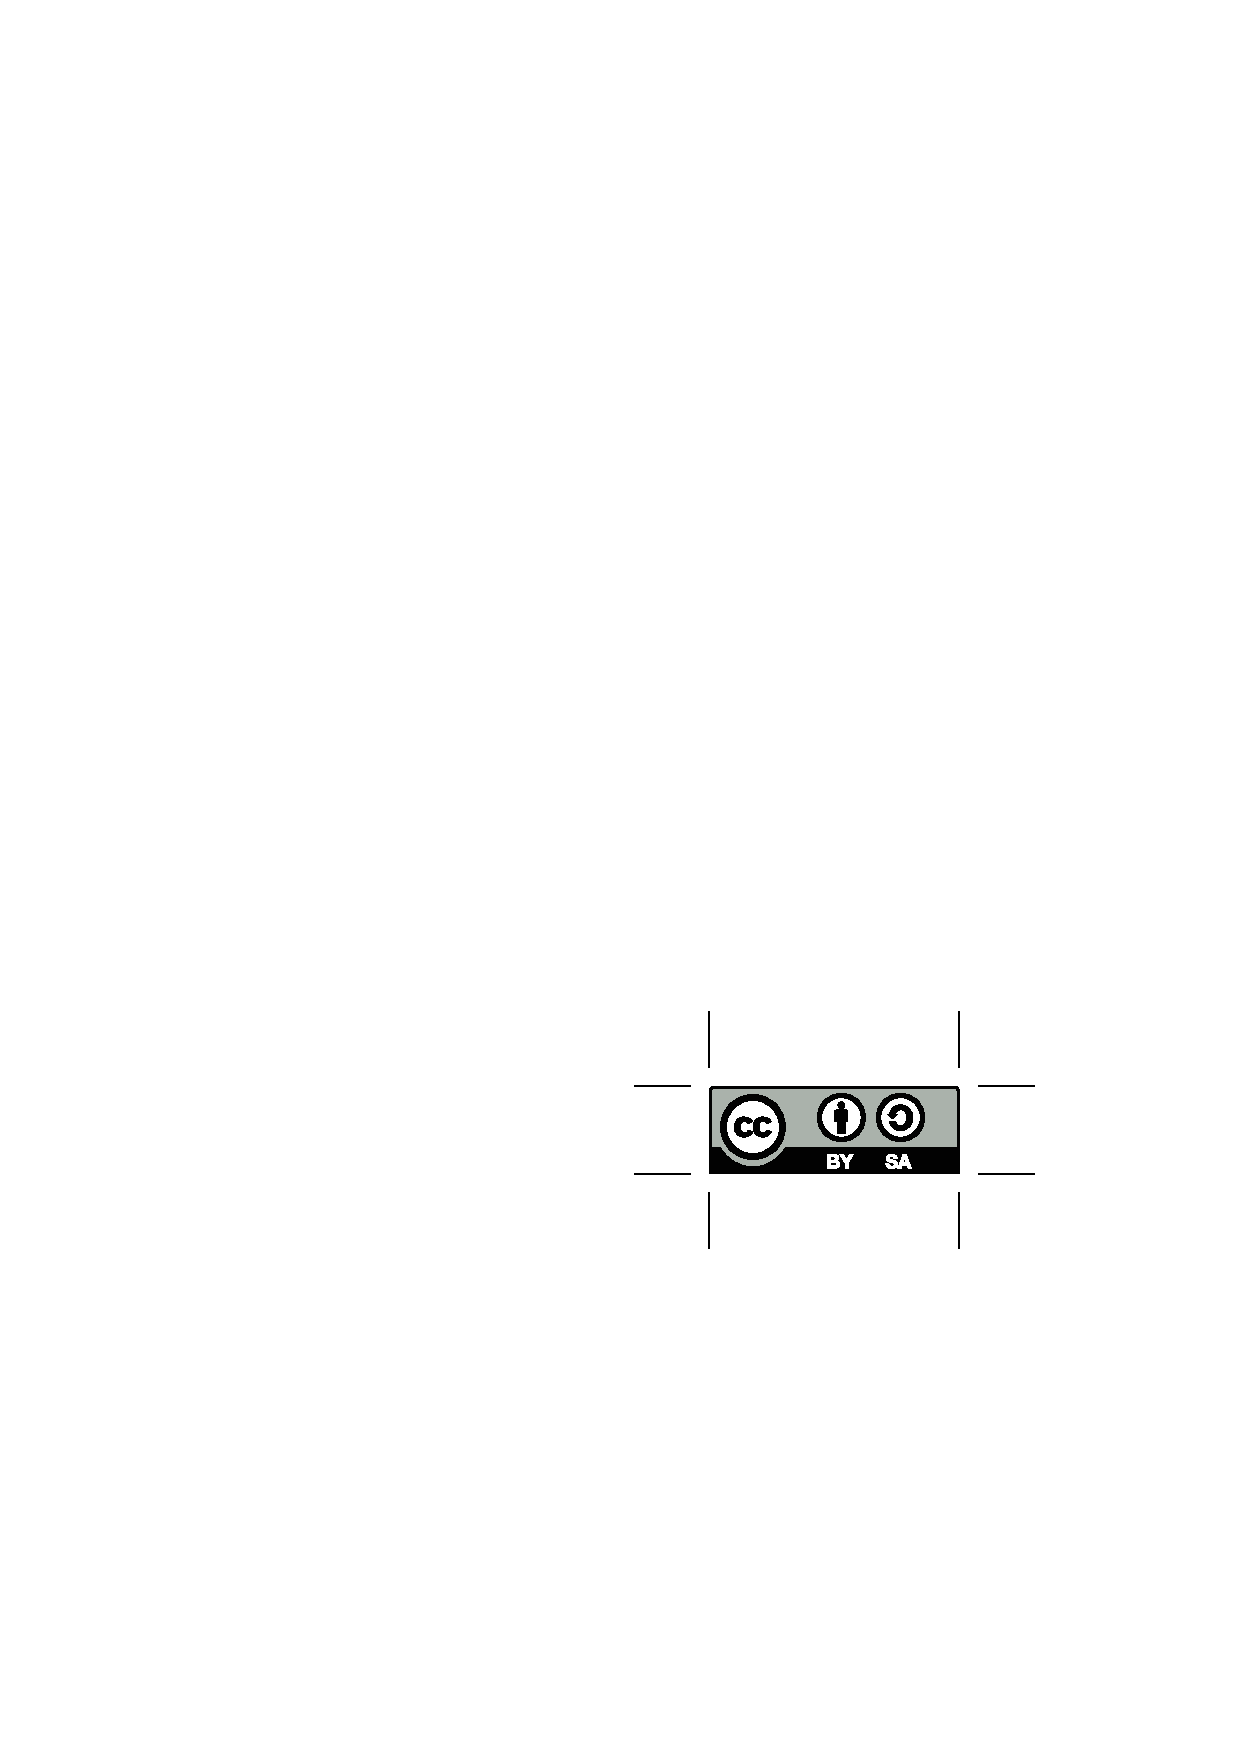
\includegraphics[scale=0.75]{by-sa}

This work is licensed under the Creative Commons Attribution-ShareAlike 4.0 International License. To view a copy of this license, visit \url{http://creativecommons.org/licenses/by-sa/4.0/} or send a letter to Creative Commons, PO Box 1866, Mountain View, CA 94042, USA. Copyright \copyright~2019-\the\year~Chika Games.

The RPG Maker trademark and copyright are property of Enterbrain, Inc. and Kadokawa Corporation. All rights belong to their respective owners.}
\newcommand{\specpreamble}{\maketitle
\tableofcontents
\newpage
\chikalegal
\newpage}


\title{RPG Maker Config File Specification (RPG\_RT.ini)}
\author{Chika Games}

\begin{document}
\specpreamble

\section{Introduction}
The \textit{RPG\_RT.ini} configuation file provides basic start-up information for RPG Maker 2000/2003 games. This file follows a simple \href{https://en.wikipedia.org/wiki/INI_file}{INI} format.

This file is found within the same directory as the RPG Maker runtime (\textit{RPG\_RT.exe}). This file is not required: if the file is not present or fields are omitted, the runtime will use default values.

\section{Data Types}
This section describes the various data types that will be used throughout this specification.

\begin{table}[h!]
\centering
\begin{tabular}{|l|l|}
\hline
\textbf{Type} & \textbf{Description}                      \\ \hline
STRING        & A string of characters.                   \\ \hline
UINT          & An unsigned integer.                      \\ \hline
BOOL          & A boolean integer: 0 is false, 1 is true. \\ \hline
\end{tabular}
\end{table}

The \textit{STRING} type has no standard encoding; the current system locale is used by the runtime. Therefore, for example, a string written in Japanese may appear incorrectly if the runtime is running on a machine with an English locale.

\section{Config File Structure}
This section details the overall structure of an \textit{RPG\_RT.ini} file.

The fields should be specified within an \textit{RPG\_RT} section. See \hyperref[sec:example]{Example Config File} for a simple example.

None of the fields listed below are required and may be omitted; missing fields will take on a default value. Fields with invalid values will be ignored and the default value will be used.

\begin{table}[h!]
\centering
\begin{tabular}{|l|l|l|l|}
\hline
\textbf{Field}  & \textbf{Type}   & \textbf{Default Value} & \textbf{Description}                                    \\ \hline
GameTitle       & \textit{STRING} & \textquote{Untitled}   & The title of the game's window.                         \\ \hline
MapEditMode     & \textit{UINT}   & 0                      & The last layer-editing mode.           \\ \hline
MapEditZoom     & \textit{UINT}   & 0                      & The last zoom-level used.              \\ \hline
FullPackageFlag & \textit{BOOL}   & False (0)              & Skip loading a runtime package. \\ \hline
\end{tabular}
\end{table}

The \textit{MapEditMode} and \textit{MapEditZoom} fields are only used by the RPG Maker editor. \textit{MapEditMode} may have the following values: 0 (lower layer), 1 (upper layer), and 2 (event layer). \textit{MapEditZoom} may have the following values: 0 (1:1 ratio), 1 (1:2 ratio), 2 (1:4 ratio), and 3 (1:8 ratio).

The \textit{FullPackageFlag} indicates whether or not a particular game is standalone or makes use of a runtime package (RTP). If this field is true (1), then an RTP is not necessary and the runtime may opt to not load one, potentially improving start-up time.

\section{Example Config File}
\label{sec:example}
Below is an example configuration file:

\begin{verbatim}
[RPG_RT]
GameTitle=My Game
MapEditMode=2
MapEditZoom=0
FullPackageFlag=1
\end{verbatim}

\textquote{My Game} will be the title of the game's window. The last time the game was edited, the editor was in the event layer, zoomed in at a 1:1 ratio. Finally, this game does not require a runtime package in order to function correctly.

\end{document}